\documentclass[a4paper,10pt]{report}
\usepackage[T1]{fontenc}
\usepackage{titlesec}
\usepackage{graphicx}
\usepackage{svg}
\usepackage{amsmath}
\usepackage{amsthm}
\usepackage{fancyvrb}
\usepackage[english]{babel}
\usepackage{csquotes}
\usepackage{hyperref}
\hypersetup{
   colorlinks=true,
   linkcolor=blue,
   urlcolor=cyan
}
\usepackage{tikz}
\usepackage{amssymb}
\usepackage[sc]{mathpazo}
\linespread{1.05}
\usepackage{microtype}
\usepackage{breqn}
\usepackage{caption}
\usepackage{subcaption}
\usepackage{minted}
\setminted{
   numberblanklines=false, 
   mathescape, 
   texcomments, 
   autogobble, 
   breakanywhere, 
   breakautoindent, 
   breaklines,
   frame=none
}
\setminted[python]{python3}
\usepackage[
   backend=biber,%
   bibencoding=utf8,%
   language=english,%
   style=numeric-comp,%
   sorting=nyt,%
   maxbibnames=10,%
   natbib=true%
]{biblatex}
\addbibresource{references.bib}
\usepackage{blkarray}
\usepackage{siunitx}
\graphicspath{ {./img/} }

% Set TOC depth and sections numbering
\setcounter{tocdepth}{3}
\setcounter{secnumdepth}{3}

% Remove chapters head and reduce spacing
\titleformat{\chapter}[hang]{\Large\bfseries}{\thechapter \hspace{2ex}}{0pt}{\Large}
\titlespacing{\chapter}{0cm}{0cm}{0.5cm}
\usepackage[parfill]{parskip}

% Make quotes italic 
\renewcommand{\mkbegdispquote}[2]{\itshape}


\begin{document}
\frenchspacing

% First page
\title{
	{{\large{\textsc{Alma Mater Studiorum $\cdot$ University of Bologna}}}}
	\rule{\textwidth}{0.4pt}\vspace{3mm}
	\textbf{Flatland Challenge} 
	\begin{figure}[!htb]
		\centering
		\includesvg[width = 200pt]{flatland-logo}
	\end{figure} \\
	Deep learning course final project
}

\author{Leonardo Calbi (\href{mailto:leonardo.calbi@studio.unibo.it}{leonardo.calbi@studio.unibo.it}) \\ Alessio Falai (\href{mailto:alessio.falai@studio.unibo.it}{alessio.falai@studio.unibo.it})}
\date{\today}
\maketitle
\newpage
\tableofcontents
\listoffigures
\newpage


\chapter*{Foreword}
The Flatland challenge is a competition organized by AIcrowd \cite{aicrowd} with the help of SBB (Swiss Federal Railways) to foster innovation with what regards the scheduling of trains trajectories in a railway environment. 

As reported on the official challenge website, SBB operates the densest mixed railway traffic in the world. It maintains and operates the biggest railway infrastructure in Switzerland: today, as of \the\year, there are more than $\num{10000}$ trains running each day, being routed over $\num{13000}$ switches and controlled by more than $\num{32000}$ signals. 

The Flatland challenge aims to address the vehicle rescheduling problem by providing a simplistic grid world environment and allowing for diverse solution approaches. In particular, the first edition of the challenge was hosted during 2019 and the submitted solutions were mainly based on OR (Operation Research) methodologies, while the second edition of the competition, i.e. the NeurIPS 2020 edition, had the goal of favoring the implementation of RL (Reinforcement Learning) based solutions.  


\chapter{Introduction}\label{chap:introduction}
At the core of this challenge lies the general vehicle rescheduling problem (VRSP) proposed by \citeauthor{vrsp} in \citeyear{vrsp} \cite{vrsp}:
\begin{displayquote}
	The vehicle rescheduling problem (VRSP) arises when a previously assigned trip is disrupted. A traffic accident, a medical emergency, or a breakdown of a vehicle are examples of possible disruptions that demand the rescheduling of vehicle trips. The VRSP can be approached as a dynamic version of the classical vehicle scheduling problem (VSP) where assignments are generated dynamically.
\end{displayquote}

The problem is formulated as a 2D grid environment with restricted transitions between neighboring cells to represent railway networks. On the 2D grid, multiple agents with different objectives must collaborate to maximize the global reward.

The overall goal is to make all agents (trains) arrive at their target destination with a minimal travel time. In other words, we want to minimize the time steps (or wait time) that it takes for each agent in the group to reach its destination.


\chapter{Background}\label{chap:background}

\subsubsection*{Railway}
As already pointed out, the Flatland environment is represented as a 2D grid of dimension $W\times H$ and each cell in the grid can be one of many different types. The different types of cells can belong to the following categories: \texttt{rail} and \texttt{empty}.

The \texttt{rail} cells are the most intricated of the two, in that there exists different types of them. In particular, figure \ref{fig:rail-cells} shows examples of possible \texttt{rail} cells that can be used to build up a railway environment in Flatland. Other than the ones shown in figure \ref{fig:rail-cells} there are also diamond crossings (i.e. two orthogonal straight rails crossing each other), single slip switches (i.e. the same as double slip switches but with a single choice) and symmetrical switches (which are special kinds of switches that bifurcate to a left and right branch). Moreover, every \texttt{rail} cell can be rotated by $90^{\circ}$ and mirrored along both axis, to allow more combinations between them to be made, in order to guarantee a great degree of diversity between different railways.

\begin{figure}[h]
	\centering
	\captionsetup[subfigure]{justification=centering}
	\begin{subfigure}[t]{.20\linewidth}
		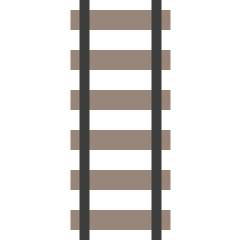
\includegraphics[width=\textwidth]{straight-rail.png}
		\caption{Straight}
		\label{fig:rail-cell-straight}
	\end{subfigure}%
    ~
	\begin{subfigure}[t]{.20\linewidth}
		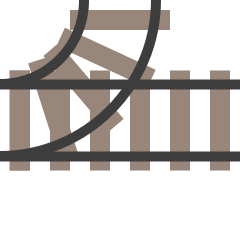
\includegraphics[width=\textwidth]{simple-switch-rail.png}
		\caption{Simple switch}
		\label{fig:rail-cell-simple}
	\end{subfigure}%
	~ 
	\begin{subfigure}[t]{.20\linewidth}
		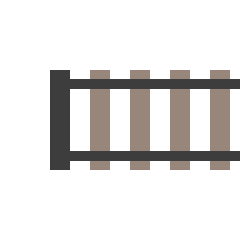
\includegraphics[width=\textwidth]{deadend-rail.png}
		\caption{Deadend}
		\label{fig:rail-cell-deadend}
	\end{subfigure}%
	~
	\begin{subfigure}[t]{.20\linewidth}
		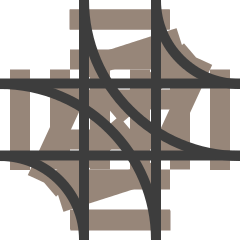
\includegraphics[width=\textwidth]{double-slip-rail.png}
		\caption{Double slip switch}
		\label{fig:rail-cell-double}
	\end{subfigure}%
    
	\caption{Different \texttt{rail} cell types}
	\label{fig:rail-cells}
\end{figure}

Moreover, \texttt{rail} cells can be occupied by the following entities (the ones shown in figure \ref{fig:agent-target}):
\begin{itemize}
	\item Agent: one \texttt{rail} cell can be seen as a resource with availability equal to one, so that in each time step only one agent can occupy it
	\item Target: each target is statically assigned to one \texttt{rail} cell. Target cells represent the destination of one or more agents (different agents could have the same target). Moreover, the number of possible targets present in the environment is clearly limited by the number of agents
\end{itemize}

\begin{figure}[h]
	\centering
	\captionsetup[subfigure]{justification=centering}
	\begin{subfigure}[t]{.25\linewidth}
		
\includegraphics[width=\textwidth]{agent.png}
		\caption{Agent}
		\label{fig:agent}
	\end{subfigure}%
    ~
	\begin{subfigure}[t]{.25\linewidth}
		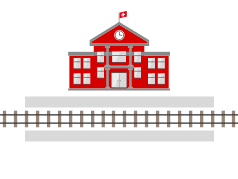
\includegraphics[width=\textwidth]{target.png}
		\caption{Target}
		\label{fig:target}
	\end{subfigure}%
	\caption{Agents and targets}
	\label{fig:agent-target}
\end{figure}

An important fact about the different types of \texttt{rail} cells is that only switches require an agent to make a choice. In Flatland (like in reality) a maximum of two options is available. There does not exist a switch with three or more options.

Finally, every cell that is not \texttt{rail} is \texttt{empty} and neither targets nor agents can fill it up. As shown in figure \ref{fig:env-example}, it is interesting to notice that Flatland is a very sparse environment, meaning that there are a lot more \texttt{empty} cells than \texttt{rail} ones: because of this, representing the environment as a simple dense matrix could lead to overheads and efficiency issues, especially when dealing with relatively big environments.

In the end, the only cell types that we care about are the \texttt{rail} ones: the \texttt{empty} ones are useful only for visualization purposes. Because of this, we could think of representing the environment as a sparse matrix or as a graph containing only \texttt{rail} cells or a subset of them (we will address this issue in section \ref{sec:railway-encoding}).

\begin{figure}[h]
	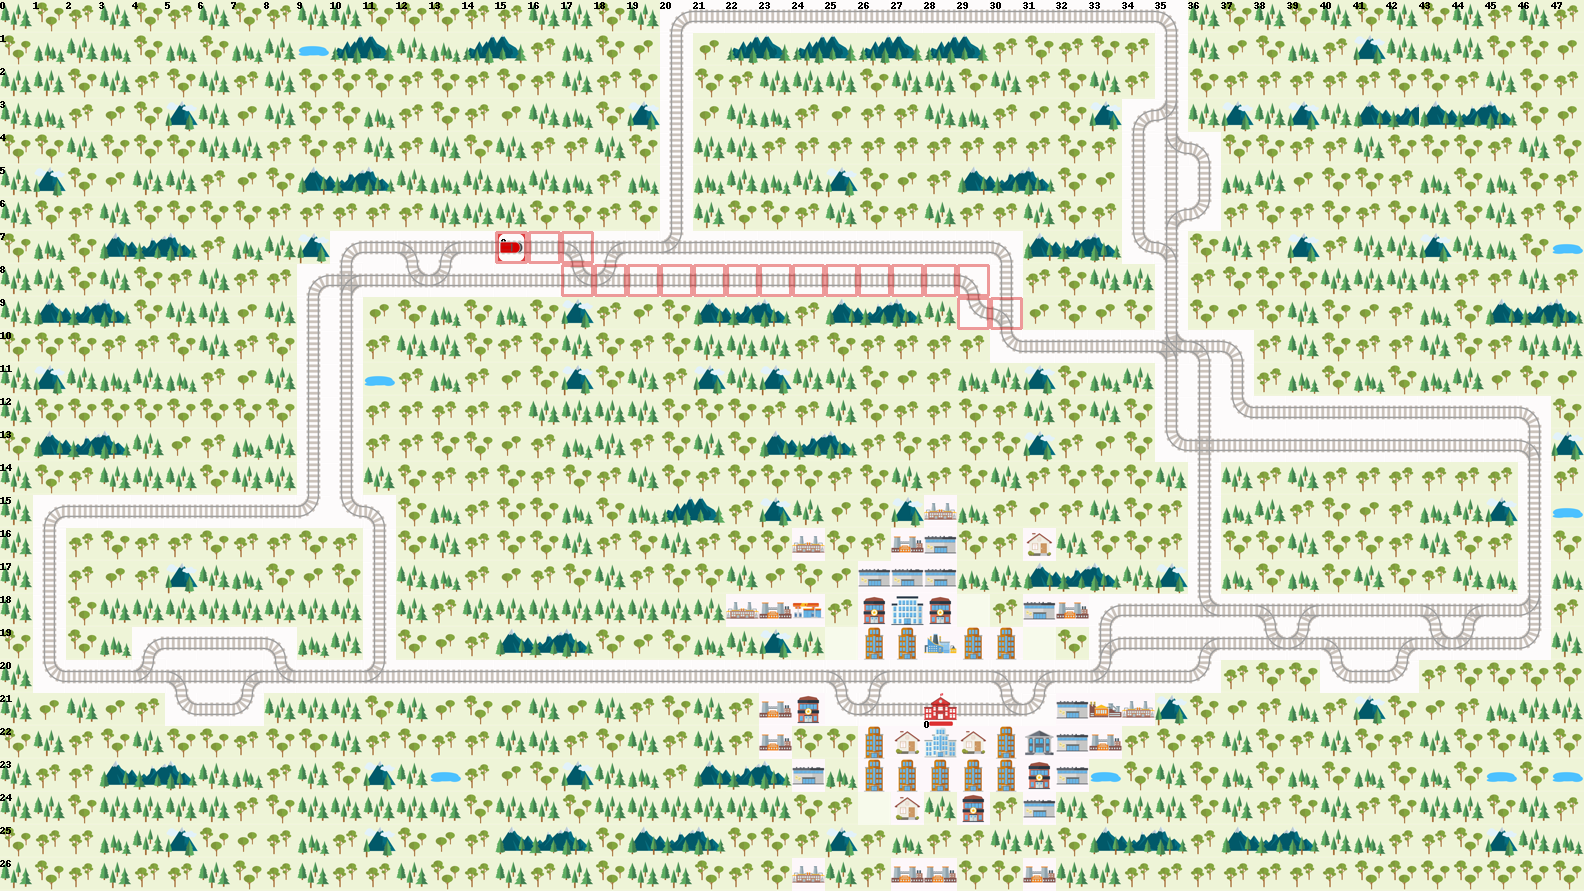
\includegraphics[width=\textwidth]{env.png}
	\caption{An example of a railway environment}
	\label{fig:env-example}
\end{figure}

\subsubsection*{Transitions}
An agent in the Flatland environment is a train that starts from a random \texttt{rail} cell in the map and has to arrive to its assigned \texttt{target} cell in the minimum number of steps. To do so, the agent can only occupy \texttt{rail} cells. 

To move from a cell to another one the agent has to make a choice and, depending on the cell type that they are on and on the connections between cells, an agent can transition from cell $i$, when looking towards direction $d_i$, to cell $j$, looking towards direction $d_j$, if and only if $T_i(d_i, d_j)=1$, where $T_i$ is the transition matrix associated to cell $i$, s.t. $T_i(d_i, d_j)=0$ means that the transition from cell $i$, direction $d_i$ to cell $j$, direction $d_j$ is forbidden (likewise $T_i(d_i, d_j)=1$ means that the transition is allowed). Directions $d_*$ are represented as the $4$ cardinal directions, i.e. North, East, South and West (N, E, S, W), so that each transition matrix $T_*$ can be characterized as a $4\times4$ binary matrix. For example, a deadend cell like the one reported in figure \ref{fig:rail-cell-deadend} would have a transition matrix like the one shown in figure \ref{fig:rail-cell-bitmap}.

\begin{figure}[h]
	\noindent\begin{minipage}{.5\linewidth}
		\begin{equation*}
			\begin{blockarray}{ccccc}
				& N & E & S & W \\
				\begin{block}{c(cccc)}
				N & 0 & 0 & 0 & 0 \\
				E & 0 & 0 & 0 & \mathbf{1} \\
				S & 0 & 0 & 0 & 0 \\
				W & 0 & 0 & 0 & 0 \\
				\end{block}
			\end{blockarray}
		\end{equation*}
	\end{minipage}%
	$\xrightarrow[\text{bitmap}]{\text{to}}$
	\begin{minipage}{.5\linewidth}
		\begin{equation*}
			0000 \; 000\mathbf{1} \; 0000 \; 0000
		\end{equation*}
	\end{minipage}
	\caption{Transition matrix and bitmap of a deadend}
	\label{fig:rail-cell-bitmap}
\end{figure}

As we can observe, only one entry in the matrix has value $1$, meaning that only one transition is possible, i.e. the one s.t. the agent enters heading East and exits heading West. 

In the Flatland library, a transition matrix is represented by a bitmap, which can be seen as a linearization by rows of the reported matrix (the mapping between the transition matrix of the deadend cell \ref{fig:rail-cell-deadend} and its bitmap is again shown in figure \ref{fig:rail-cell-bitmap}). In this way, by simply counting the number of true values in the bitmap, we can understand the type of \texttt{rail} cell that we are examining (e.g. only one true value indicates a deadend, while exactly two true values indicate a straight rail). 

\subsubsection*{Actions}
Flatland has a discrete action space, meaning that only $5$ possibilities have to be considered at each transition. In particular, Flatland uses the following convention:
\begin{enumerate}
	\item \texttt{MOVE_FORWARD}: the agent maintains the current movement direction, if possible (i.e. if it was heading North, it will continue heading North)
	\item \texttt{MOVE_LEFT}: if the agent is at a switch with a transition to its left, the agent will choose the left path, otherwise the action has no effect (e.g. if the agent was heading North, it will be directed towards East)
	\item \texttt{MOVE_RIGHT}: if the agent is at a switch with a transition to its right, the agent will choose the right path, otherwise the action has no effect (e.g. if the agent was heading North, it will be directed towards West)
	\item \texttt{STOP_MOVING}: the agent remains in the same cell
	\item \texttt{DO_NOTHING}: the agent performs the same action as the last time step
\end{enumerate}

Usually, only a handful of the reported actions can be perfomed on a given cell, meaning that most of the times the actual number of choices is much less than $5$ (we will address this issue in section \ref{sec:choices}).

\subsubsection*{Complications}
The main complications of the Flatland challenge are given by speed profiles, conflicts and malfunctions. In particular, about speed profiles, each and every agent could have a different velocity. The standard speed (and the maximum one) is $1$, which means that the agent crosses one cell in one time step. Speeds can have values in range $(0, 1]$: if an agent has speed $s$, it means that it needs $\lceil\frac{1}{s}\rceil$ time steps to transition from one cell to the next one. 

Speeds are assigned to agents based on a custom probability mass function, so that $P(S=s)$ represents the probability that the speed $S$ of an agent is equal to $s$. For example, we could have the following \textit{pmf} (representing a uniform distribution over values $\{\frac{1}{4}, \frac{1}{3}, \frac{1}{2}, 1\}$):

\begin{equation}
	\begin{cases} 
		P(S=s) = 0.25 & \text{if } s \in \{\frac{1}{4}, \frac{1}{3}, \frac{1}{2}, 1\} \\
		P(S=s) = 0 & \text{otherwise}
	\end{cases}
\end{equation}

Clearly, the speed factor is a critical one to observe when trying to minimize the total number of time steps in a multi-agent scenario: for example, different agents have to understand that faster ones should go first if a decision has to be made. This is because we would like to avoid bottlenecks of any kind inside the railway network and slower agents can definitely become an issue in an environment with relatively long sequences of straight rails.

About the second complications, i.e. malfunctions, agents can experience defects or failures which do not let them go on in their path towards the target. A malfunction in the Flatland environment is modeled by a Poisson distribution $1 - P_{\lambda}(n=0)=1 - \frac{\lambda^{n}}{n!}\cdot e^{-\lambda}=1 - e^{-\lambda}$, where $\lambda \in (0, 1]$ is the malfunction rate s.t. $\frac{1}{\lambda}$ represents the mean frequency of occurrence of malfunctioning events. For example, if malfunctions are to be expected once every $80$ time steps for an agent, then $\lambda=\frac{1}{80}=0.0125$ and the probability of a malfunction in each time step is equal to $1-e^{-0.0125}=0.01$, while if malfunctions are more rare (e.g. once every $200$ time steps), then we would have a probability value of $1-e^{-0.005}=0.004$. Once an agent is malfunctioning, it stays so for a random number of time steps, bounded by parameters indicating the minimum and maximum duration of a malfunction period.

Again, the malfunction factor is critical, in that it could prevent one or more agents from reaching their targets in the minimum number of time steps. In this way, transitions in the environment become stochastic, thus leading to a slower and much more difficult optimization procedure.

About the third complication, i.e. conflicts, we can define it as a state in which agents cannot perform any action, because they are "blocked" by one or more neighboring agents. Different conflicting situations can arise in practice, where the most basic one is given by two agents heading in different directions in a sequence of straight rails (see figure \ref{fig:two-deadlock}): this situation can in turn cause other deadlocks to happen, as shown in figure \ref{fig:three-deadlock}.

\begin{figure}[h]
	\centering
	\captionsetup[subfigure]{justification=centering}
	\begin{subfigure}[t]{.4\linewidth}
		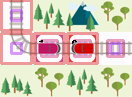
\includegraphics[width=\textwidth]{two-deadlock.png}
		\caption{Two agents}
		\label{fig:two-deadlock}
	\end{subfigure}%
    ~
	\begin{subfigure}[t]{.4\linewidth}
		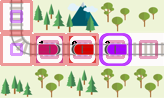
\includegraphics[width=\textwidth]{three-deadlock.png}
		\caption{Three agents}
		\label{fig:three-deadlock}
	\end{subfigure}%

	\caption{Examples of deadlocks}
	\label{fig:deadlocks}
\end{figure}

A full deadlock situation is a state in which every agent is in deadlock: in that case, no agent would be able to arrive at its target. These blocking situations are one of the most intricate and complex factors that should be addressed when designed autonomous agents in the Flatland environment, since they are quite frequent (and they get more frequent as the number of agents increases and the dimension of the grid decreases) and have disastrous consequences (at least in a real-world scenario).

Differently from malfunctions, deadlocks totally prevent agents from reaching their destination: when a malfunction occurs, agents that could previously reach their targets will still be able to reach them once the malfunction period is over, while when a conflict occurs, at least two agents will never arrive at their targets.

\chapter{Environment}
In this chapter we are going to explore better ways to encode the Flatland environment and how agents can interact with these representations.

\section{Railway encoding}\label{sec:railway-encoding}
As already described in chapter \ref{chap:background}, the default Flatland representation was not built with the goal of efficiency in mind, since it stores each and every cell of the 2D grid, while only \texttt{rail} cells are the ones that are actually used by agents. An alternative and more efficient representation could be to use some kind of sparse matrix implementation, where \texttt{empty} cells are not stored at all, but this would only be beneficial from the point of view of memory occupancy, while the usage of more specific data structures could also improve other aspects, like the computation of shortest paths from the agent's position to its target.

In this work, we decided to rely on a graph structure. In particular, we were inspired by the great work described in \cite{jonas} where the author presents the so called Cell Orientation Graph (COG), in which nodes represent cells in the 2D grid as a triple $(x, y, d)$, where $(x, y)$ are the coordinates in the grid (origin in the top-left corner with x-axis looking right and y-axis looking down) and $d$ is one of the four cardinal directions (representing the direction of entrance in the cell). In this way, one \texttt{rail} cell is represented by at most $4$ nodes in the graph: this could seem like a major drawback, but in practice we can observe that the number of nodes is roughly equivalent to the number of cells in the corresponding grid, since we got rid of the \texttt{empty} ones. 

Instead, edges in the graph are directed and represent legal transitions, so that no transition matrix or bitmap has to be stored in each node: it is simply encoded in the topology of the network. Moreover, the usage of directed edges greatly simplifies the computation of paths between nodes in the graph.

In order to further simplify the representation of the Flatland environment, we decided to entirely delete nodes which represented straight rails (with the exception of keeping straight rails containing targets and deadends). In this way, what we end up with is something that could be defined a Cell Orientation Junction Graph (COJG), since the remaining nodes are the ones in which an agent either has to make a decision or finishes its trip.

Because of the deletion of almost all nodes associated to straight rails, edges actually represent a connection between an interesting cell and another one (e.g. they link a junction to a target or a junction to a second junction). In order to maintain the same topology as before, the number of deleted straight rails between each pair of interesting nodes is used as the weight of the edge connecting them, so that the computation of shortest paths can automatically take that into account.

Figure \ref{fig:grid-cog-cojg-32x16} shows the comparison, in terms of visual representations, of the standard grid environment and both COG and COJG graphs, in a $32\times 16$ map. In table \ref{table:grid-cog-cojg-32x16} we show the improvements that can be gained by leveraging the usage of the Cell Orientation Graph, and in particular of its modified version, i.e. the Cell Orientation Junction Graph, by computing the number of nodes, edges and \texttt{empty} cells in each representation, in the same $32\times 16$ map of figure \ref{fig:grid-cog-cojg-32x16}. 

\begin{figure}[h]
	\centering
	\captionsetup[subfigure]{justification=centering}
	\begin{subfigure}[b]{.8\linewidth}
		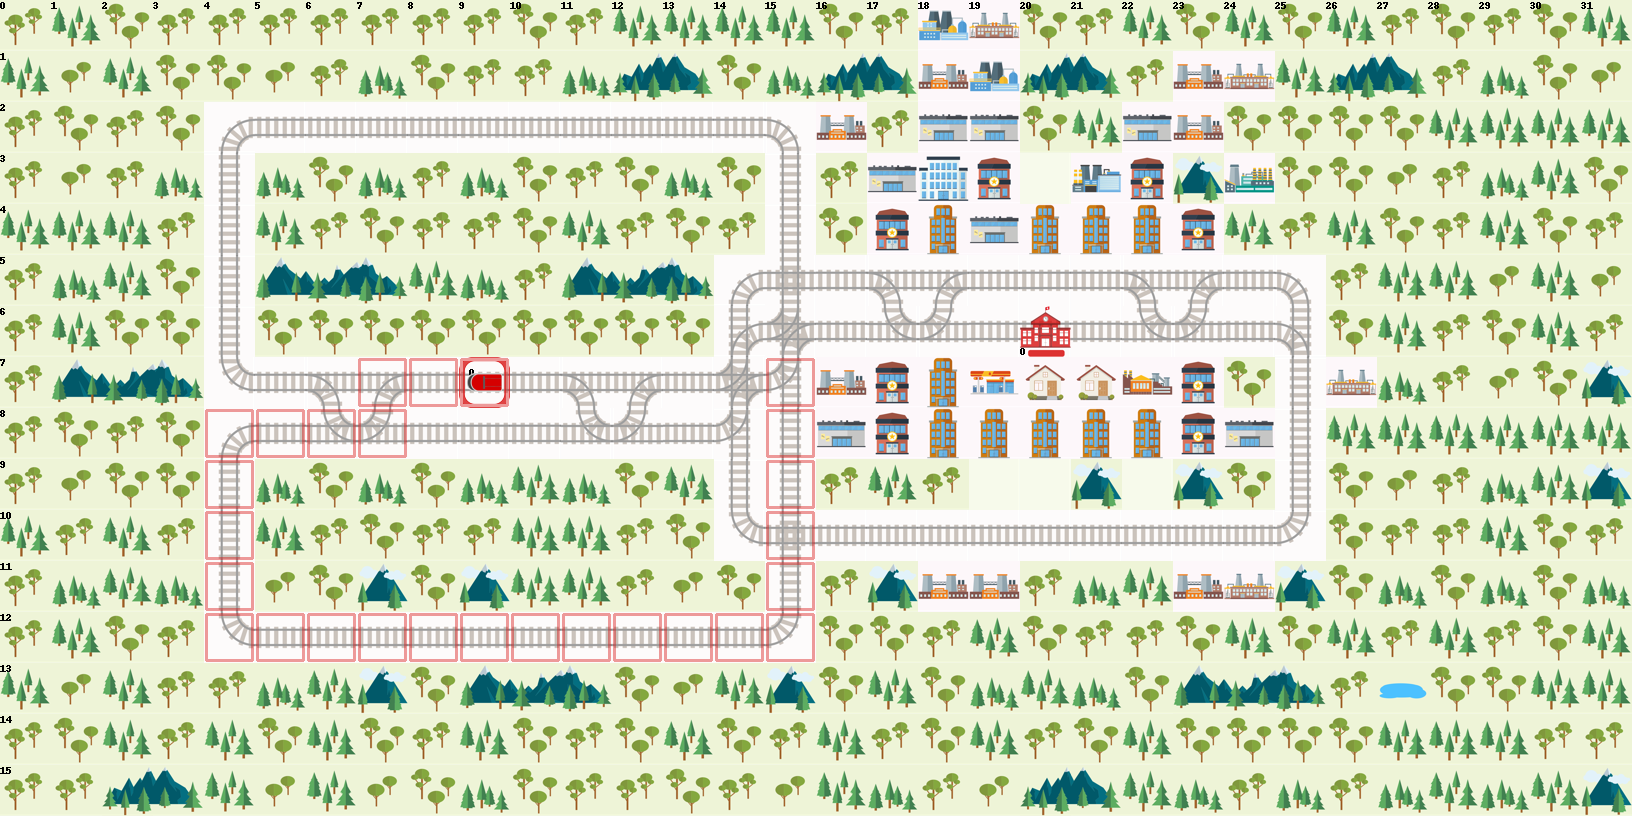
\includegraphics[width=\textwidth]{grid-env-32x16.png}
		\caption{Grid}
		\label{fig:grid-env-32x16}
	\end{subfigure}%
    
	\begin{subfigure}[b]{.8\linewidth}
		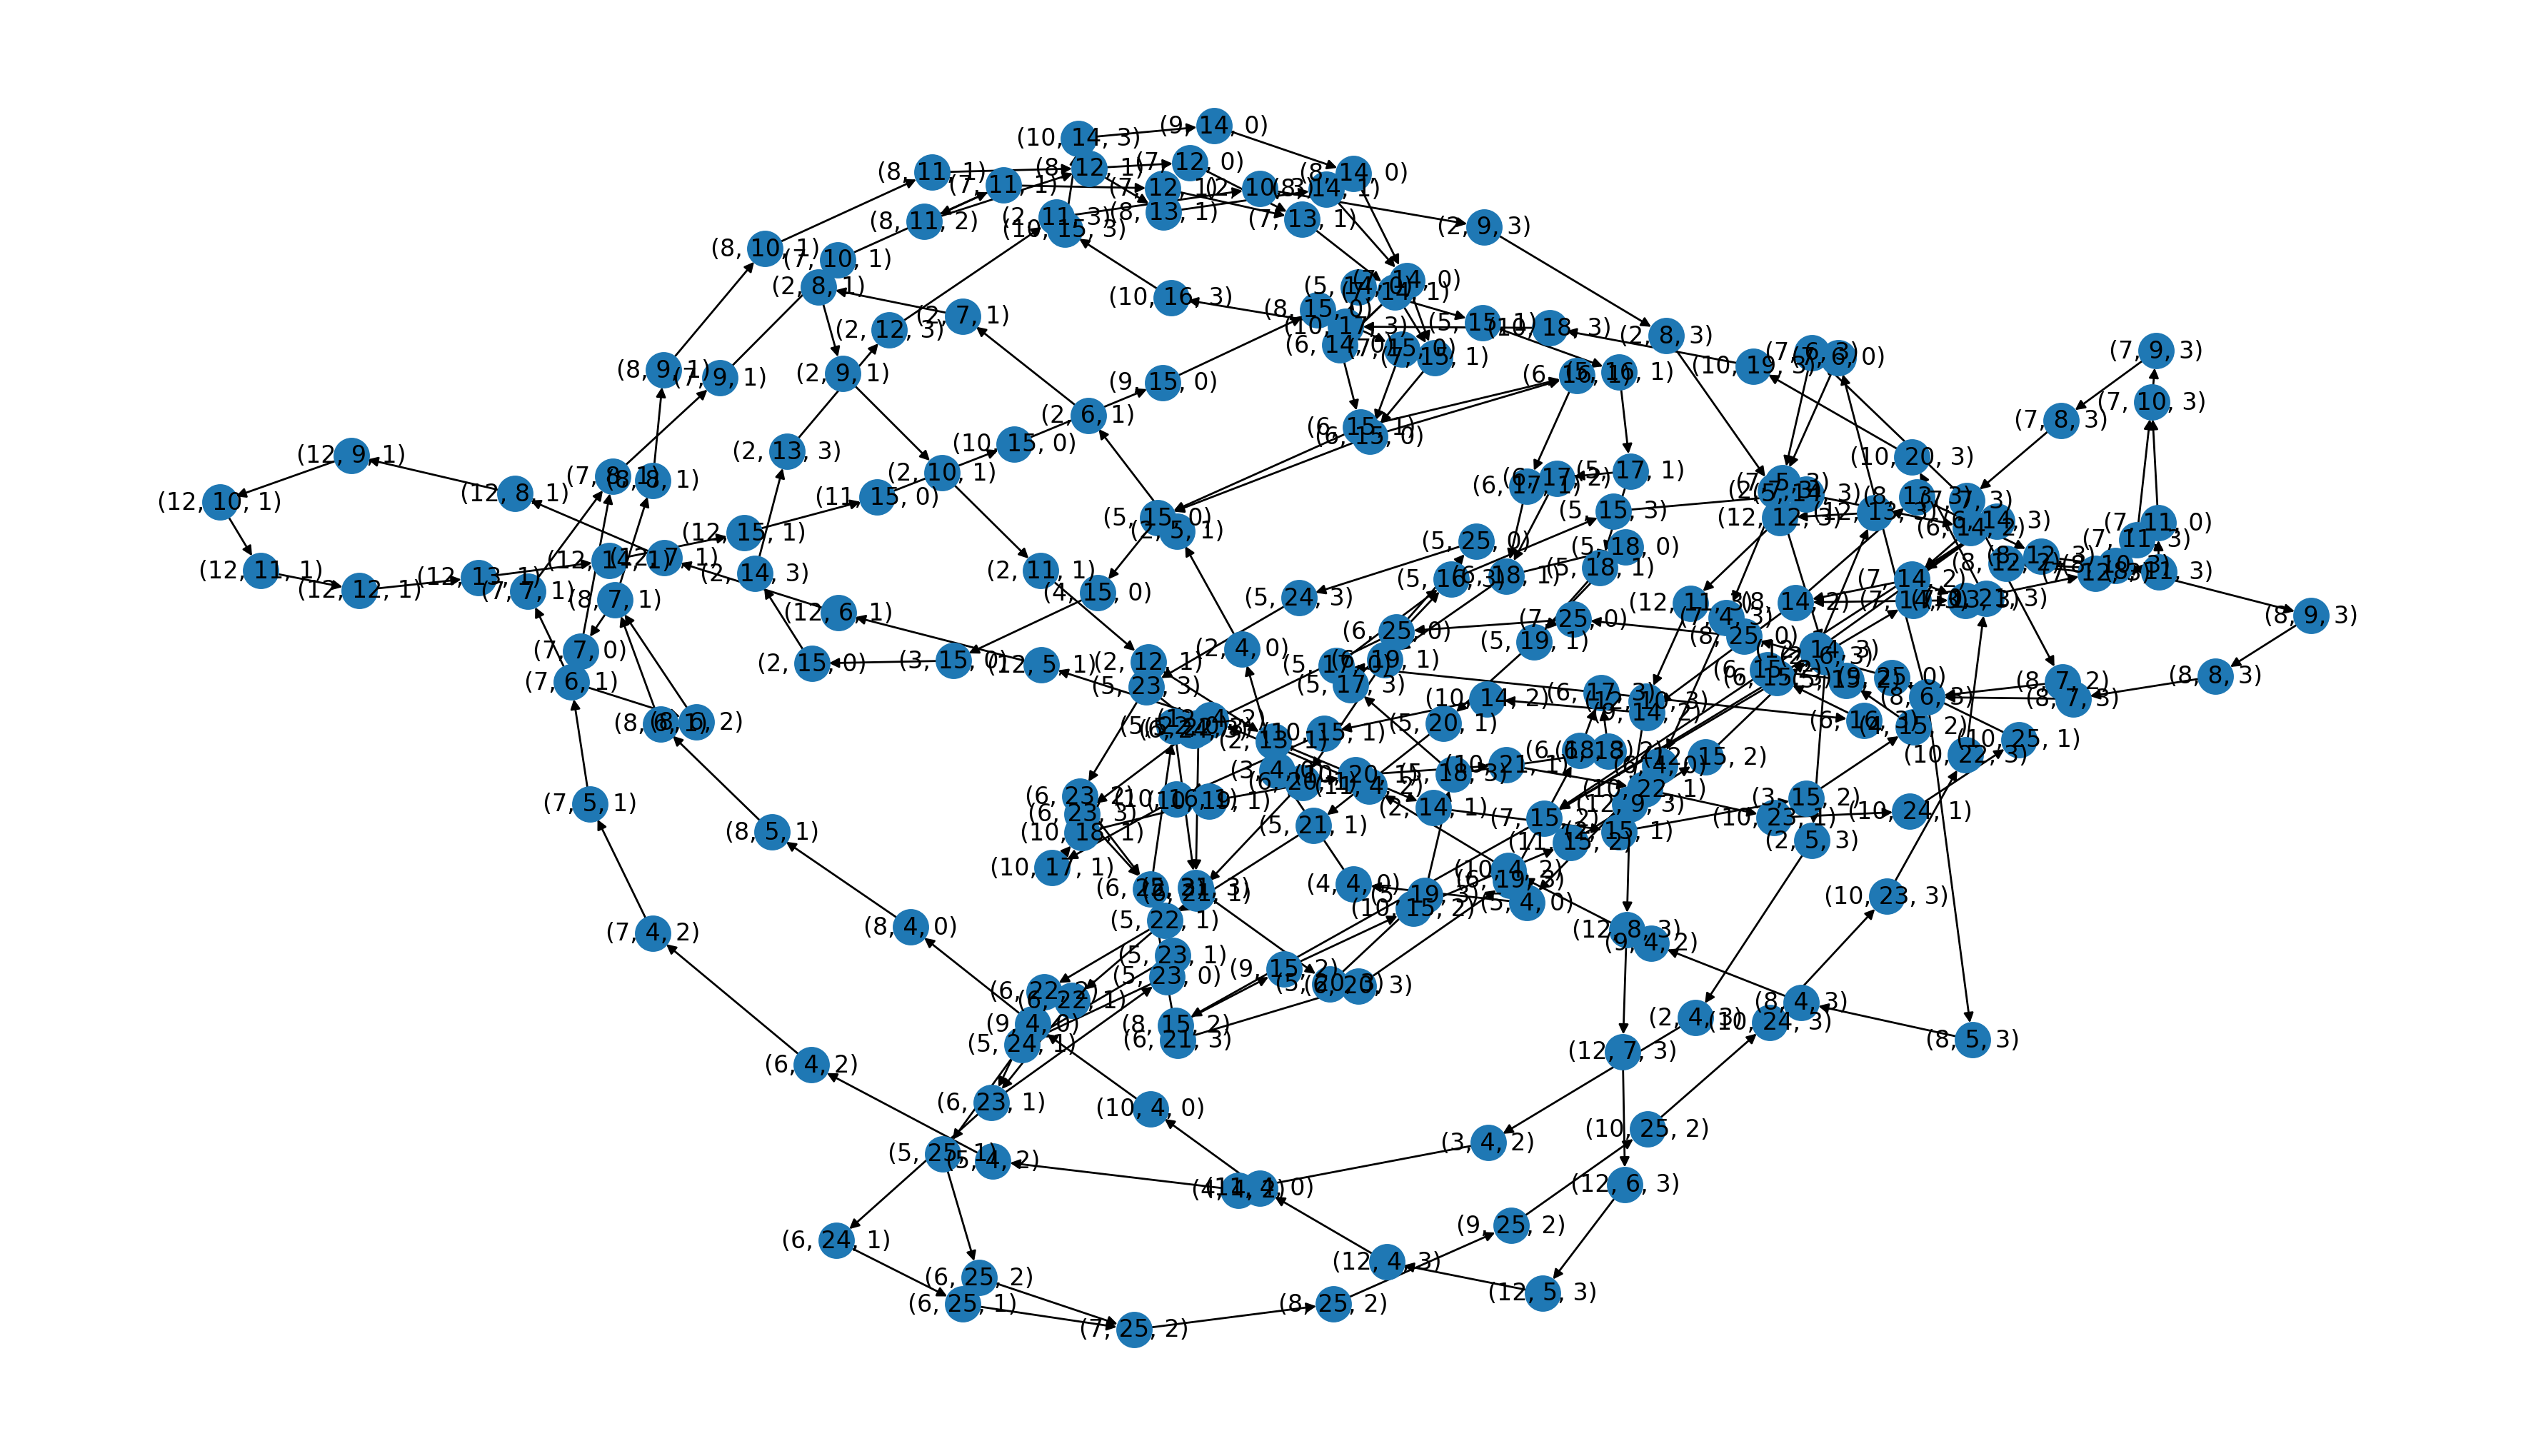
\includegraphics[width=\textwidth]{cog-env.png}
		\caption{COG}
		\label{fig:cog-env-32x16}
	\end{subfigure}%
	
	\begin{subfigure}[b]{.8\linewidth}
		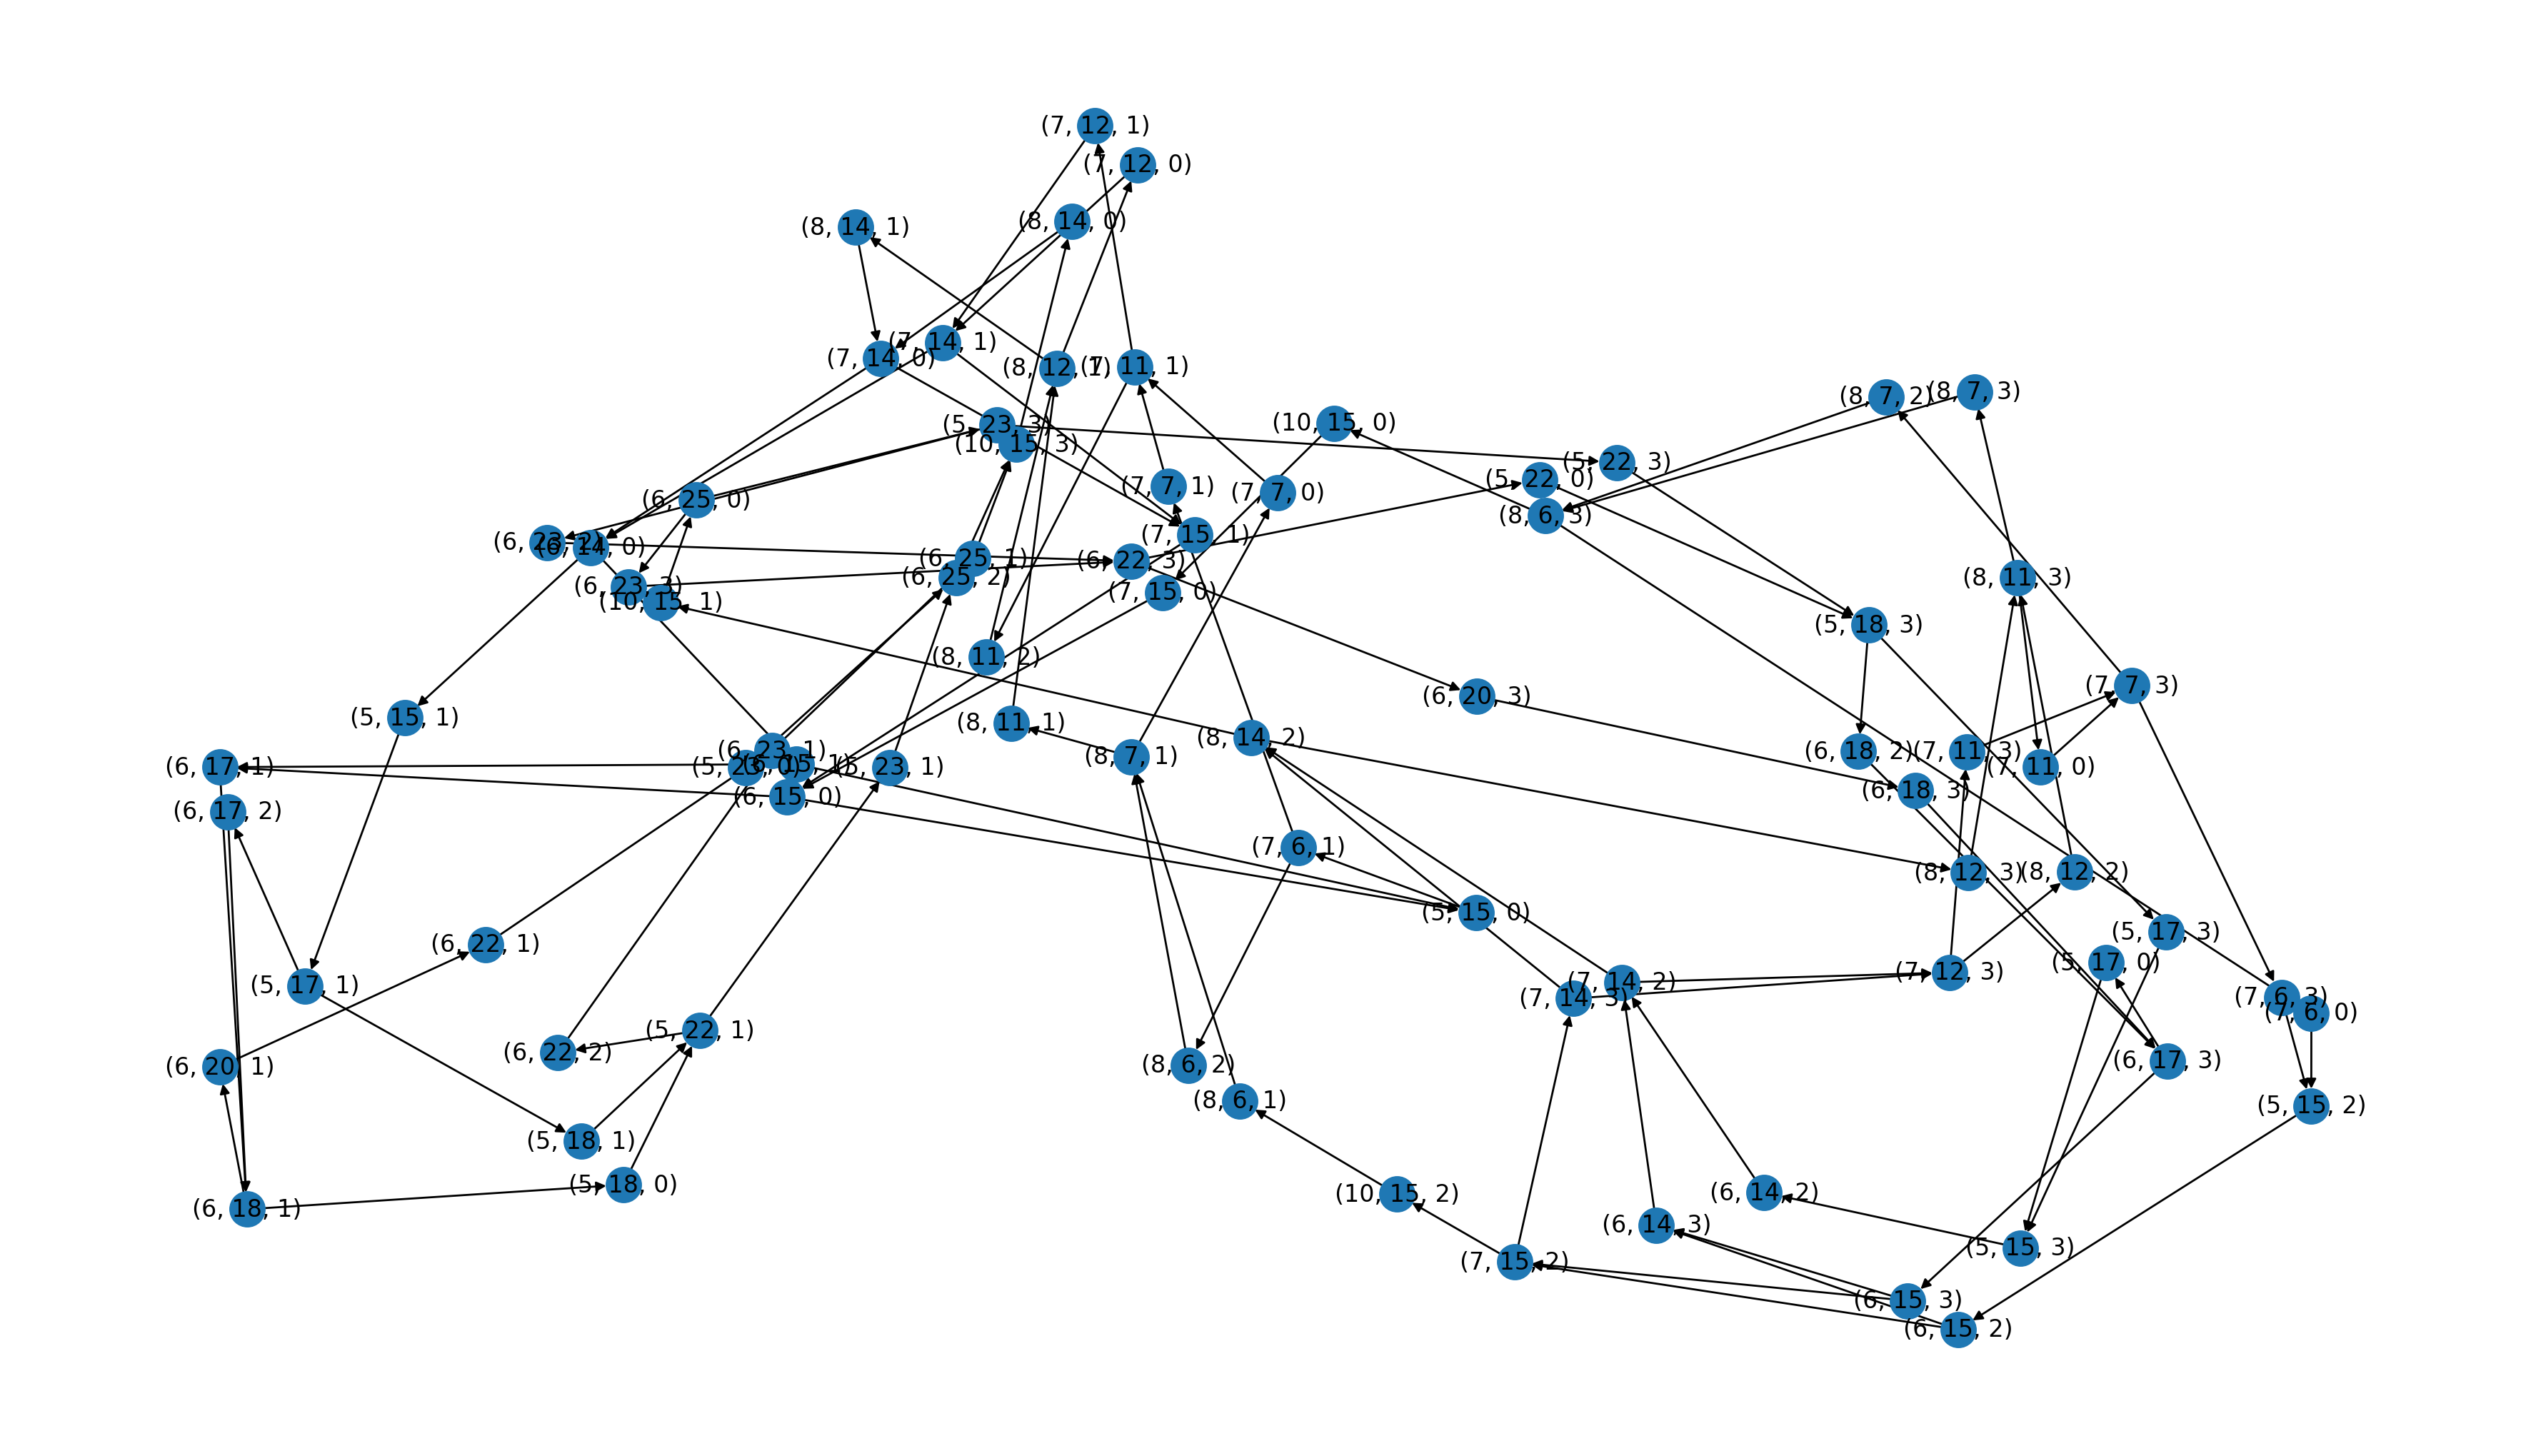
\includegraphics[width=\textwidth]{cojg-env.png}
		\caption{COJG}
		\label{fig:cojg-env-32x16}
	\end{subfigure}%

	\caption{Different railway encodings of a $32\times 16$ map}
	\label{fig:grid-cog-cojg-32x16}
\end{figure}

\begin{table}[h]
	\center
	\begin{tabular}{||c c c c||} 
		\hline
		& \textbf{Nodes} & \textbf{Edges} & \textbf{Empty} \\ [0.5ex] 
		\hline\hline
		\textbf{Grid} & 512 & - & \num{413} \\ 
		\hline
		\textbf{COG} & 226 & 254 & 0 \\
		\hline
		\textbf{COJG} & 78  & 106 & 0 \\
		\hline
   \end{tabular}
   \caption{Grid, COG, COJG comparison in a $32\times 16$ map}
   \label{table:grid-cog-cojg-32x16}
\end{table}

Since a $32x16$ map is too small to observe big improvements, in figure \ref{fig:grid-cog-cojg-128x64} we also report another example of a sparse grid environment of dimension $128\times64$ and we compare it with its encodings in table \ref{table:grid-cog-cojg-128x64}.

\begin{figure}[h]
	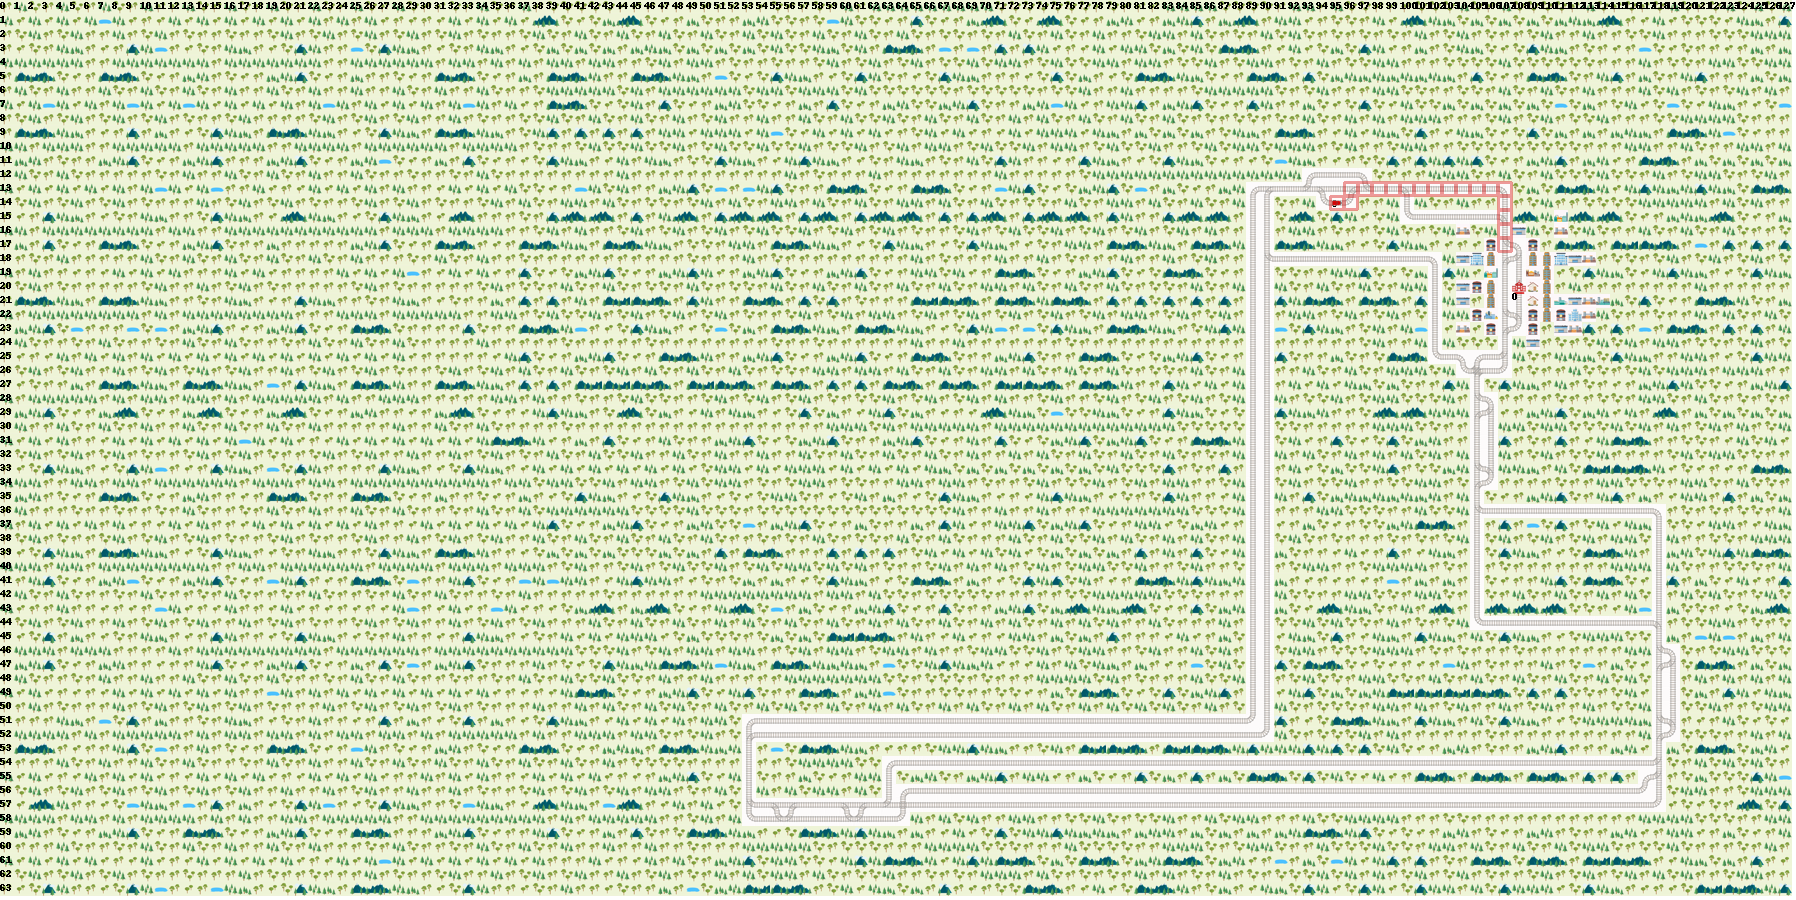
\includegraphics[width=\textwidth]{grid-env-128x64.png}
	\caption{Sparse $128\times64$ grid environment}
	\label{fig:grid-cog-cojg-128x64}
\end{figure}

\begin{table}[h]
	\center
	\begin{tabular}{||c c c c||} 
		\hline
		& \textbf{Nodes} & \textbf{Edges} & \textbf{Empty} \\ [0.5ex] 
		\hline\hline
		\textbf{Grid} & \num{8192} & - & \num{7732} \\ 
		\hline
		\textbf{COG} & 1050 & 1096 & 0 \\
		\hline
		\textbf{COJG} & 136  & 182 & 0 \\
		\hline
   \end{tabular}
   \caption{Grid, COG, COJG comparison in a $128\times 64$ map}
   \label{table:grid-cog-cojg-128x64}
\end{table}
 
\section{Predictions}
As reported in Flatland official FAQs, because railway traffic is limited to rails, many decisions that an agent has to take need to consider future situations and detect upcoming conflicts ahead of time. Therefore, Flatland provides the possibility of predictors that predict where agents will be in the future. The stock predictor simply assumes that each agent travels along its shortest path.

\subsection{Shortest and deviation paths}
One of the key advantages of COJG is that it enables us to apply standard shortest path algorithms on directed weighted graphs without any kind of overhead. In particular, we decided to use Dijkstra's algorithm since we do not have negatively weighted edges (in that case, Dijkstra's algorithm could get stuck in a cycle containing at least one edge with negative weight, since it may cycle an infinite number of times and sometimes go down with the total cost as much as it likes). 

To build our predictor, we took inspiration from the standard predictor given by the Flatland library as a baseline, which computes shortest paths directly on the 2D grid representation. Our predictor instead takes into account two possibilities: an agent either follows its shortest path or deviates from it. The computation of shortest paths is incremental, meaning that once it is done it only gets updated (i.e. the first node is removed). The only event that causes a re-computation of the shortest path is when the agent makes a choice that does not follow the stored path.

Deviation paths are instead computed on the fly and they represent alternatives from each node of the shortest path. The computation of deviation path $i$, given the shortest path $n_1, \dots, n_i, n_{i+1}, \dots, n_d$, is simply another call to the Dijkstra's routine, where edge $(n_i, n_{i+1})$ is forbidden. In this example, $d$ represents the maximum depth of both shortest and deviation paths.

In this way, the prediction becomes a list of paths, where the first one is the shortest path, composed by at most $d$ nodes, and the following ones are $d-1$ deviation paths, still composed by at most $d$ nodes. When an agent is relatively close to its target (i.e. less than $d$ nodes away from it), the actual path could have a dimension which is less than $d$: to avoid troubles when dealing with dynamically sized vectors, paths are padded to the full depth with special symbols.

In case an agent cannot reach its target anymore, the prediction only comprises a path of two nodes, i.e. the agent's position and the next node in the COJG graph. This mini-path is stored because predictions are used to compute possible deadlocks and, even if an agent cannot arrive at its target anymore, it is still present in the railway environment and it could be a possible source of conflicts.

\section{Observations}
\subsection{Tree}
\subsection{Binary tree}
\section{Choices}\label{sec:choices}
\section{Rewards shaping}

\chapter{Policy}
\section{Action masking}
\section{Action selection}
\subsection{$\epsilon$-greedy}
\subsection{Boltzmann}
\section{Replay buffers}
\subsection{Uniform}
\subsection{Prioritized}

\chapter{DQN}
\section{Architectures}
\subsection{Vanilla}
\subsection{Double}
\subsection{Dueling}
\section{Bellman equation}
\subsection{Max}
\subsection{Softmax}

\chapter{GNN}

\chapter{Results}



\chapter{Conclusions}

\printbibliography

\end{document}
